\chapter{Introduction}
\section{Unboxing}
Open the packing box and take out the robot arm, control box, power cable, accessory package and other products.

\section{Safety Guidelines}
\label{sec:安全指南}
Before installing and powering up the robot, please read this section carefully for the correct installation order and starting method.

\subsection{Safety Warning Symbols}

\dange{When this symbol appears, please pay special attention to the conditions in the warning statement that may lead to electrical hazards. Failure to pay attention may result in injury, death, or equipment damage.}

\danger[Danger/Warning]{When this symbol appears, please pay special attention to the situations in the warning statement that may lead to personal safety and equipment damage. Failure to pay attention may result in personal injury, death, or severe equipment damage.}

\info{When this symbol appears, please pay attention to the matters that need attention during the operation. Failure to pay attention may result in faulty operation and accidental injury.}

\subsection{Environmental Conditions for Installation}
Before installing the robot, check whether the environmental conditions meet the following requirements, so as to avoid malfunction of the robot or accidental injury.

\begin{itemize}
\item Ambient temperature: $0\sim 40\oC$
\item Ambient relative humidity: $25\%\sim 85\%$
\item Surrounding environment: no corrosive gas or liquid, no oily smoke or salt spray, no dust or metal chips, no radioactive materials, no flammable materials, no electromagnetic noise, no radioactive materials, and try to avoid direct sunlight.
\item Workspace: sufficient space for safe work must be ensured (drag-and drop teaching, maintenance, etc.).
\item Mounting surface: When installing the robot, choose a sturdy and shock­proof surface that can withstand at least 10 times the full torsion force of the base joint (the maximum torque of the base joint is $40 \Nm$) and at least 5 times the weight of the robot (the body weight of the robot is $9.5 \kg$).
\end{itemize}

\info{\begin{itemize}[leftmargin=1.5em]
	\item Operating environment: Avoid water, dust and oily fume. If put in similar scenes, the equipment shall be shielded.
	\item Do not disassemble the machine. Otherwise, product damage may result.
	\item During the disassembly and assembly process of the product, handle it gently to prevent bumping and dropping.
\end{itemize}}

% \clearpage

\danger{The robot needs to be safely placed on a solid shock­ proof surface. Please ensure that the operation of the robot will not be affected by impact or vibration. Otherwise, the loosening of the robot installation screws may cause the robot to tip over, causing accidental injury or property damage.}
\danger{Please ensure that there is no flammable gas, flammable dust, and flammable liquid, etc. in the installation environment, otherwise an explosion or a fire may result.}
\danger{Please ensure that there is no water, corrosive gas, metal shavings, dust, etc. in the installation environment, and ensure that the temperature and humidity of the installation environment are within the allowable range, otherwise it may cause the robot to malfunction, break down or leak electricity.}
\danger{Do not use it in an environment that exceeds the range of the robot's anti­electromagnetic interference, electrostatic discharge capability, etc., otherwise it may cause the robot to shut down or change its trajectory, resulting in unpredictable danger. \ footnote{See \prettyref{app:参照标准}} for details.}

% \clearpage

\subsection{Extra Notices}
The control box should be placed horizontally, and there should be at least $5 \cm$ gaps between the air inlets and outlets on both sides to ensure air circulation and heat dissipation.

\dange{The control box and cables should avoid contact with any liquid. Do not touch the plug with wet hands, otherwise electric shocks, even casualties may result.}

\danger{The control box must not be exposed to dust or a humid environment that exceeds the IP20 protection level. Pay close attention to the environment with conductive dust.}

% \vfill

% \section{产品简介}

\section{Product Composition}

The LM3 Robot is mainly composed of a robot arm and a control box. The robot arm has 6 rotary joints, i.e. 6 degrees of freedom (DoF). As shown in \prettyref{fig:机器人关节示意图}, the robot joints include a base (joint 1), a shoulder (joint 2), an elbow (joint 3), wrist 1 (joint 4), wrist 2 (joint 5) and wrist 3 (joint 6).

\begin{figure}[ht]
    \centering
    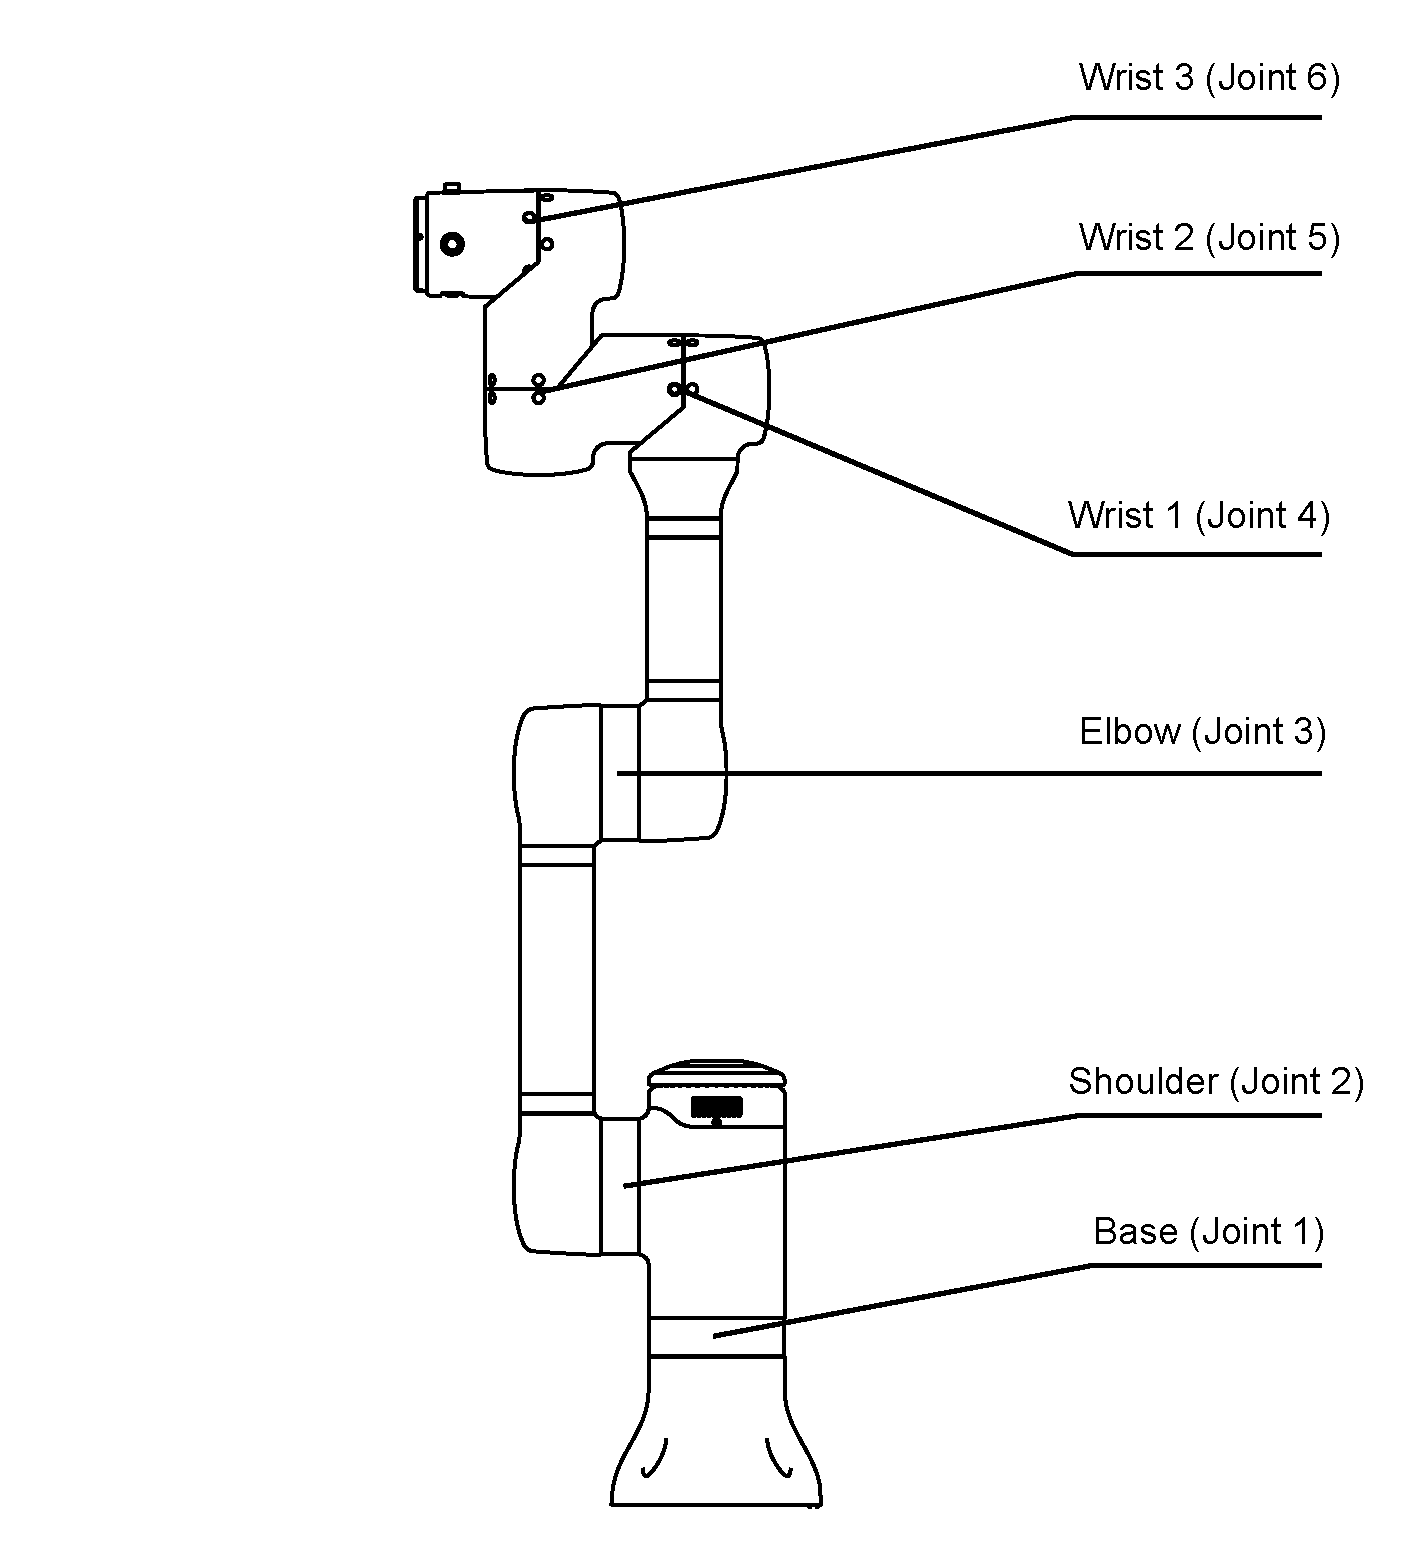
\includegraphics[height=8cm]{image/arms.pdf}
    \caption{Robot Joints}
    \label{fig:机器人关节示意图}
\end{figure}

The robot arm (hereinafter referred to as {\itshape the robot}) is the actuator of the robot product. The base is where the robot is installed. The shoulder and elbow can perform larger movements. Wrist 1 and wrist 2 can perform more precisely, and wrist 3 can connect the end effectors.

% \clearpage

The control box is the control part of the robot system, which can control the position and posture of the robot in the workspace, and connect the electrical input and output terminals of the equipment. %
To ensure safe operation in practical applications, an emergency stop button (optional) is usually externally connected to the control box. %
For convenient usage, an external power button (optional) can also be connected.

As shown in \prettyref{fig:机器人本体及控制箱连接}, the control box is connected to the robot via the robot cable. After connecting and powering up\footnote{Please refer to \prettyref{cha:基础操作}.}, users can access the robot's \LM \footnote{\LM is a robot control system tailored by {\TheCompany} for the robot. All visual operations and control of the robot must be performed after logging into the \LM system.} system  to control the robot via the browser \footnote{It is recommended to use Google Chrome, Microsoft Edge or other modern browsers based on the Webkit kernel to get a better user experience.} of a computer, tablet, mobile phone or other terminals, and view various status information of the robot.

\begin{figure}[h!]
    \centering
    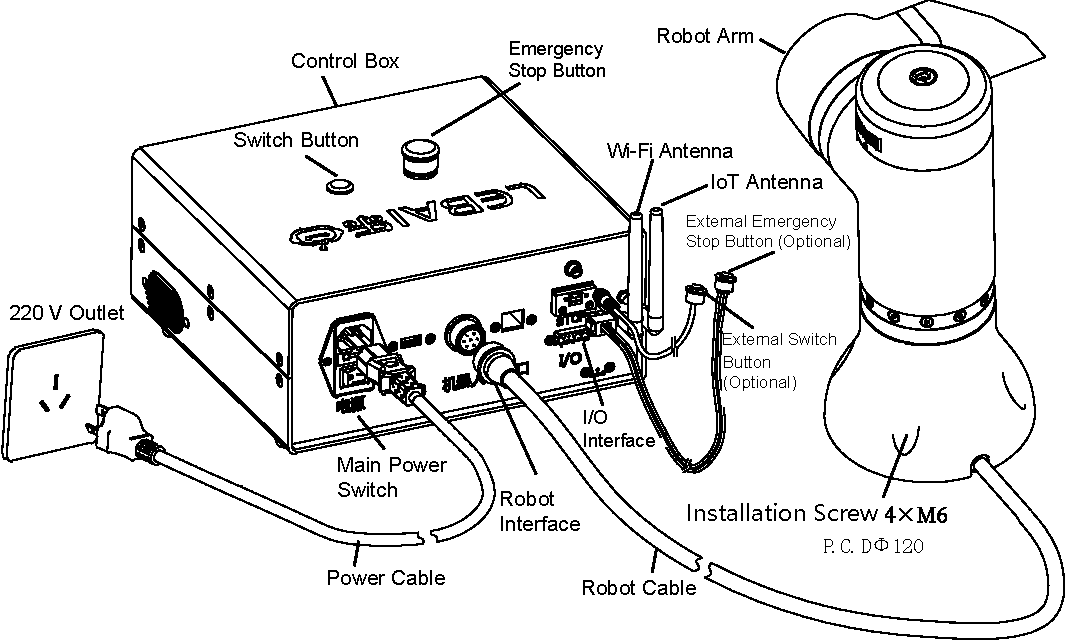
\includegraphics[width=0.9\textwidth]{en/image/robot_links.pdf}
    \caption{Robot and control box}
    \label{fig:机器人本体及控制箱连接}
\end{figure}

% \clearpage

\section{Technical Specifications}

See \prettyref{tab:机器人基础参数} and \prettyref{tab:控制箱基础参数}.

% \begin{table}[htb!]
%     \centering
%     \rowcolors{1}{trEven}{trOdd}
%     \newcommand\Thr[1]{\cellcolor{th}\sffamily\color{white}{#1}}
%     \begin{tabular}{cllll}
% \tO & \Thr{自由度} & 6 & \Thr{工作半径} &		$638\mm $ \\
% \tO & \Thr{有效负载   } &	$\le 3\kg$ & \Thr{重量   } &	$9.5\kg$\\
% \tO & \Thr{重复精度   } &	$\pm 0.5\mm$ & \Thr{末端速度   } &	$\le 2\unit{m/s}$\\
% \tO & \Thr{环境湿度   } &	$25\sim 85\%$(无冷凝) & \Thr{环境温度} &	$0\sim 40\oC$\\
% \tO & \Thr{防护等级} &	IP54 & \Thr{供电电源} &	$48\unit{V}$(DC)\\
% \multirow{-6}{4em}{\tO 机器人} & \Thr{安装方式   } &	正装、倒装、侧装 & \Thr{安装面积   } &	$\approx 160 \unit{cm^2}$\\
% \tE & \Thr{尺寸} & $270\times 250\times 130(H) \mm$ & \Thr{重量} & $3.8\kg$ \\
% \tE & \Thr{机器人电缆长度} & $2\unit{m}$ & \Thr{供电电源} & $100\sim 240\unit{V}$(AC), $50\sim 60\unit{Hz}$ \\
% \multirow{-3}{4em}{\tE 控制箱} & \Thr{防护等级} & IP20 & \Thr{通讯协议} & 以太网  \\
%     \end{tabular} 
% \footnotesize{控制箱和机器人整机典型功耗	$150\unit{W}$}
%     \caption{乐白机器人基础参数}
%     \label{tab:基础参数}
% \end{table}

\begin{table}[htb!]
    \centering
    \rowcolors{1}{trOdd}{trEven}
    \caption{Technical specifications of the control box}
    \label{tab:控制箱基础参数}
    \begin{tabular}{ll}    
    \Thr{Size} & $270\times 250\times 130(H) \mm$ \\
    \Thr{Weight} & $3.8\kg$ \\
    \Thr{Power supply} & $100\!\sim\! 240\unit{V}$(AC), $50\!\sim\! 60\unit{Hz}$ \\
    \Thr{Cable length} & $2\unit{m}$ \\
    \Thr{Protection level} & IP20 \\
    \Thr{Protocol} & Ethernet  \\
    \end{tabular}
    
    \tablenote{The typical power consumption of the control box and the robot is $130\unit{W}$}
    \end{table}
    
\begin{table}[htb!]
    \centering
    \rowcolors{1}{trOdd}{trEven}
    \caption{Technical specifications of the robot}
    \label{tab:机器人基础参数}
    \begin{tabular}{ll}
\Thr{DoF} & 6 \\
 \Thr{Working radius} &		$638\mm $ \\
\Thr{Payload} &	$\le 3\kg$ \\
 \Thr{Weight} &	$9.5\kg$\\
\Thr{Repeatability} &	$\pm 0.5\mm$ \\
 \Thr{TCP Speed} &	$\le 2\unit{m/s}$\\
\Thr{Ambient humidity} &	$25\!\sim\! 85\%$ \\
 \Thr{Ambient temperature} &	$0\!\sim\! 40\oC$\\
\Thr{Protection level} &	IP54 \\
 \Thr{Power supply} &	$48\unit{V}$(DC)\\
\Thr{Install directions} &	Up, Down and Side \\
 \Thr{Installation area} &	$\approx 160 \unit{cm^2}$\\
    \end{tabular}
\end{table}

\clearpage

Technical specifications of the control box is shown in \prettyref{tab:控制箱电气规范}:

\begin{table}[ht]
    \centering\small
    \rowcolors{1}{trEven}{trOdd}
    \caption{Technical specifications of the control box}
\newcommand{\fenlei}[2][trEven]{\multirow{-2}{5em}{\cellcolor{#1}\minitab[c]{\cellcolor{#1}#2}}}
\begin{tabular}{lllll}
\rowcolor{th} \Th{Parameters}    & \Th{Minimum}    & \Th{Typical}  & \Th{Maximum}  & \Th{Unit}\\
Nominal Voltage	&	100	&	220	&	240	&	V(AC)\\
External Utility Fuse	&	18	&	20	&	22	&	A\\
% 外部市电保险丝\footnotemark[a]	&	18	&	20	&	22	&	A\\
% 外部市电保险丝\footnotemark[b]	&	18	&	20	&	22	&	A\\
Input Frequency	&	47	&	50	&	63	&	Hz\\
Nominal Operating Power	&	90	&	130	&	400	&	W\\
\end{tabular}
% \tablenote{At $100\sim 240\unit{V}$}
	\label{tab:控制箱电气规范}
\end{table}

% \vfill

% \clearpage

\section{Joints}

% \vspace*{-1cm}
See \prettyref{tab:运动轴}。

\begin{table}[htb!]
    \centering
    \rowcolors{1}{trEven}{trOdd}
    \def\dps{\unit{^\circ/s}}
    \caption{Lebai robot joints}
    \label{tab:运动轴}
    \begin{tabular}{ccc}
\rowcolor{th} \Th{Joint} &	\Th{Motion limit} &	\Th{Maximum speed}\\
Joint 1   &	Unlimited  &	$180\dps$ \\
Joint 2   &	Unlimited  &	$180\dps$ \\
Joint 3   &	Unlimited  &	$180\dps$ \\
Joint 4   &	Unlimited  &	$180\dps$ \\
Joint 5   &	Unlimited  &	$180\dps$ \\
Joint 6   &	Unlimited  &	$180\dps$ \\
    \end{tabular}

    \tablenote{The joint rotation range is unlimited mentioned above exclude the robot's self­interference. Due to the actual motion scene, the self­interference conditions can be different.}
\end{table}

% \vspace{-10pt}

% \clearpage

\clearpage

% \vfill

\section{Workspace}
\label{sec:工作空间}

\begin{figure}[htb!]
    \centering
    \subfigure[Along the $Z$ axis]{
    	\begin{minipage}[b]{0.4\textwidth}\centering
   		 	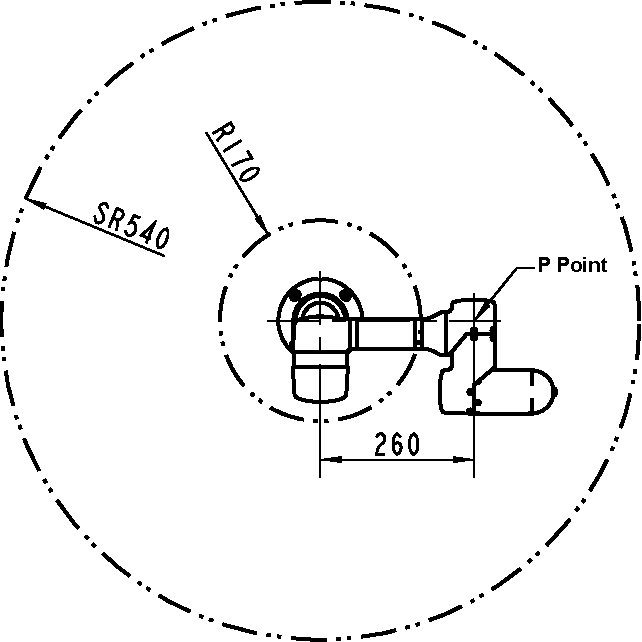
\includegraphics[width=\linewidth]{en/image/view-via-z.pdf}
    	\end{minipage}
    }
    \subfigure[Along the $X$ or $Y$ axis]{
    	\begin{minipage}[b]{0.4\textwidth}\centering
   		 	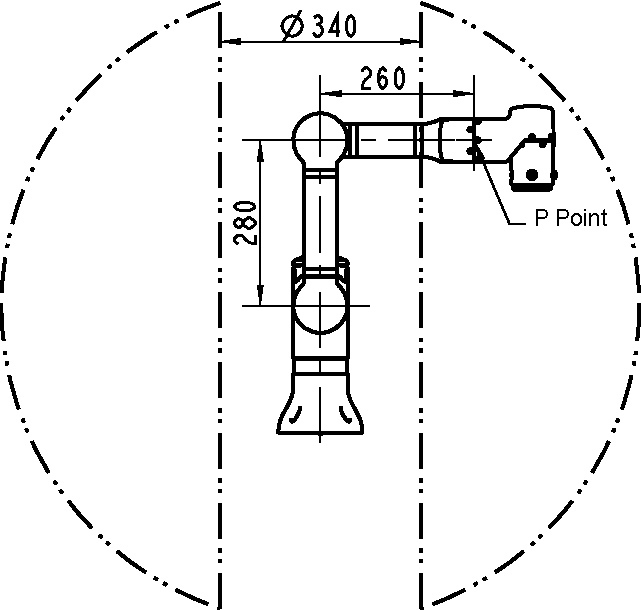
\includegraphics[width=\linewidth]{en/image/view-via-xy.pdf}
    	\end{minipage}
    }
    \caption{Schematic diagram of Lebai robot workspace}
    \label{fig:机器人运动范围}
\end{figure}

The workspace of the LM3 Robot refers to the area circled with a radius of $540\mm$ around the base joint. As shown in \prettyref{fig:机器人运动范围}, the range shown by the two­dot chain line is the best operating area of point $\!P\!$.

\clearpage

\section{I/O}

The I/O provided by LM3 consists of two parts: the control box and the flange. According to different application scenarios, you can choose the I/O at different locations to implement the corresponding I/O operation.

% \vfill

\begin{enumerate}
    \item As shown in \prettyref{fig:控制箱IO} and \prettyref{tab:控制箱IO}, the robot control box provides:
    \begin{itemize}
        \item 4 digital inputs, 4 digital outputs.
        \item 2 analog inputs, 2 analog outputs.
    \end{itemize}

\begin{figure}[htb!]
    \centering
    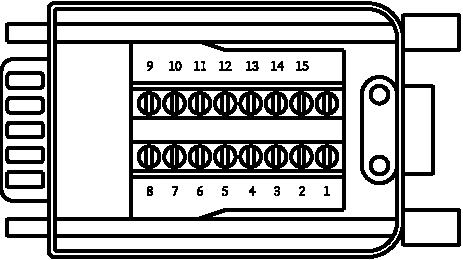
\includegraphics[height=4cm]{en/image/robot_box_io_plugin.pdf}
    \caption{Schematic diagram of the control box I/O hardware port}
    \label{fig:控制箱IO}
\end{figure}

% \vspace{-1cm}

% \newpage

\begin{table}[htb!]
    \centering
    % \rowcolors{1}{trEven}{trOdd}
\caption{Control box I/O description}
\begin{tabular}{cll}
\rowcolor{th} \Th{Index}	&  \Th{Function}	& \Th{Parameters}\\
\tO  1	& \tO Positive pole	& \tO $24\unit{V}$  \\
\tE  2	& \tE Analog output 1 & \tE \\
\tO  3	& \tO Analog output 2 & \multirow{-2}{5cm}{\tE Voltage: output $0\sim 10\unit{V}$\\Current:  output $4\sim 20\unit{mA}$}\\
\tE  4	& \tE Digital  output 1	& \tO \\
\tO  5	& \tO Digital  output 2	& \tO \\
\tE  6	& \tE Digital  output 3	& \tO \\
\tO  7	& \tO Digital  output 4	& \multirow{-4}{5cm}{\tO PNP, output voltage $24\unit{V}$\\Total maximum current $2\unit{A}$}\\
\tE  8	& \tE Negative pole	& \tE \\
\tO  9	& \tO Analog input 1 & \tO \\
\tE  10	& \tE Analog input 2	& \multirow{-2}{5cm}{\tO Voltage: input $0\sim 10\unit{V}$\\Current: input $4\sim 20\unit{mA}$}\\
\tO  11	& \tO Digital input 1	& \tE \\
\tE  12	& \tE Digital input 2	& \tE \\
\tO  13	& \tO Digital input 3	& \tE \\
\tE  14	& \tE Digital input 4	& \multirow{-4}{5cm}{\tE PNP, input voltage $3\sim 30\unit{V}$}\\
\tO  15	& \tO Negative pole	& \tO \\
% \tE GND & \tE & \tE \\
\end{tabular}
\label{tab:控制箱IO}
\end{table}

\clearpage

    \item As shown in \prettyref{fig:法兰盘IO} and \prettyref{tab:法兰盘IO}, provided on the end flange:
    \begin{itemize}
        \item 2 digital inputs.
        \item 2 digital outputs.
    \end{itemize}

\begin{figure}[htb!]
    \centering
    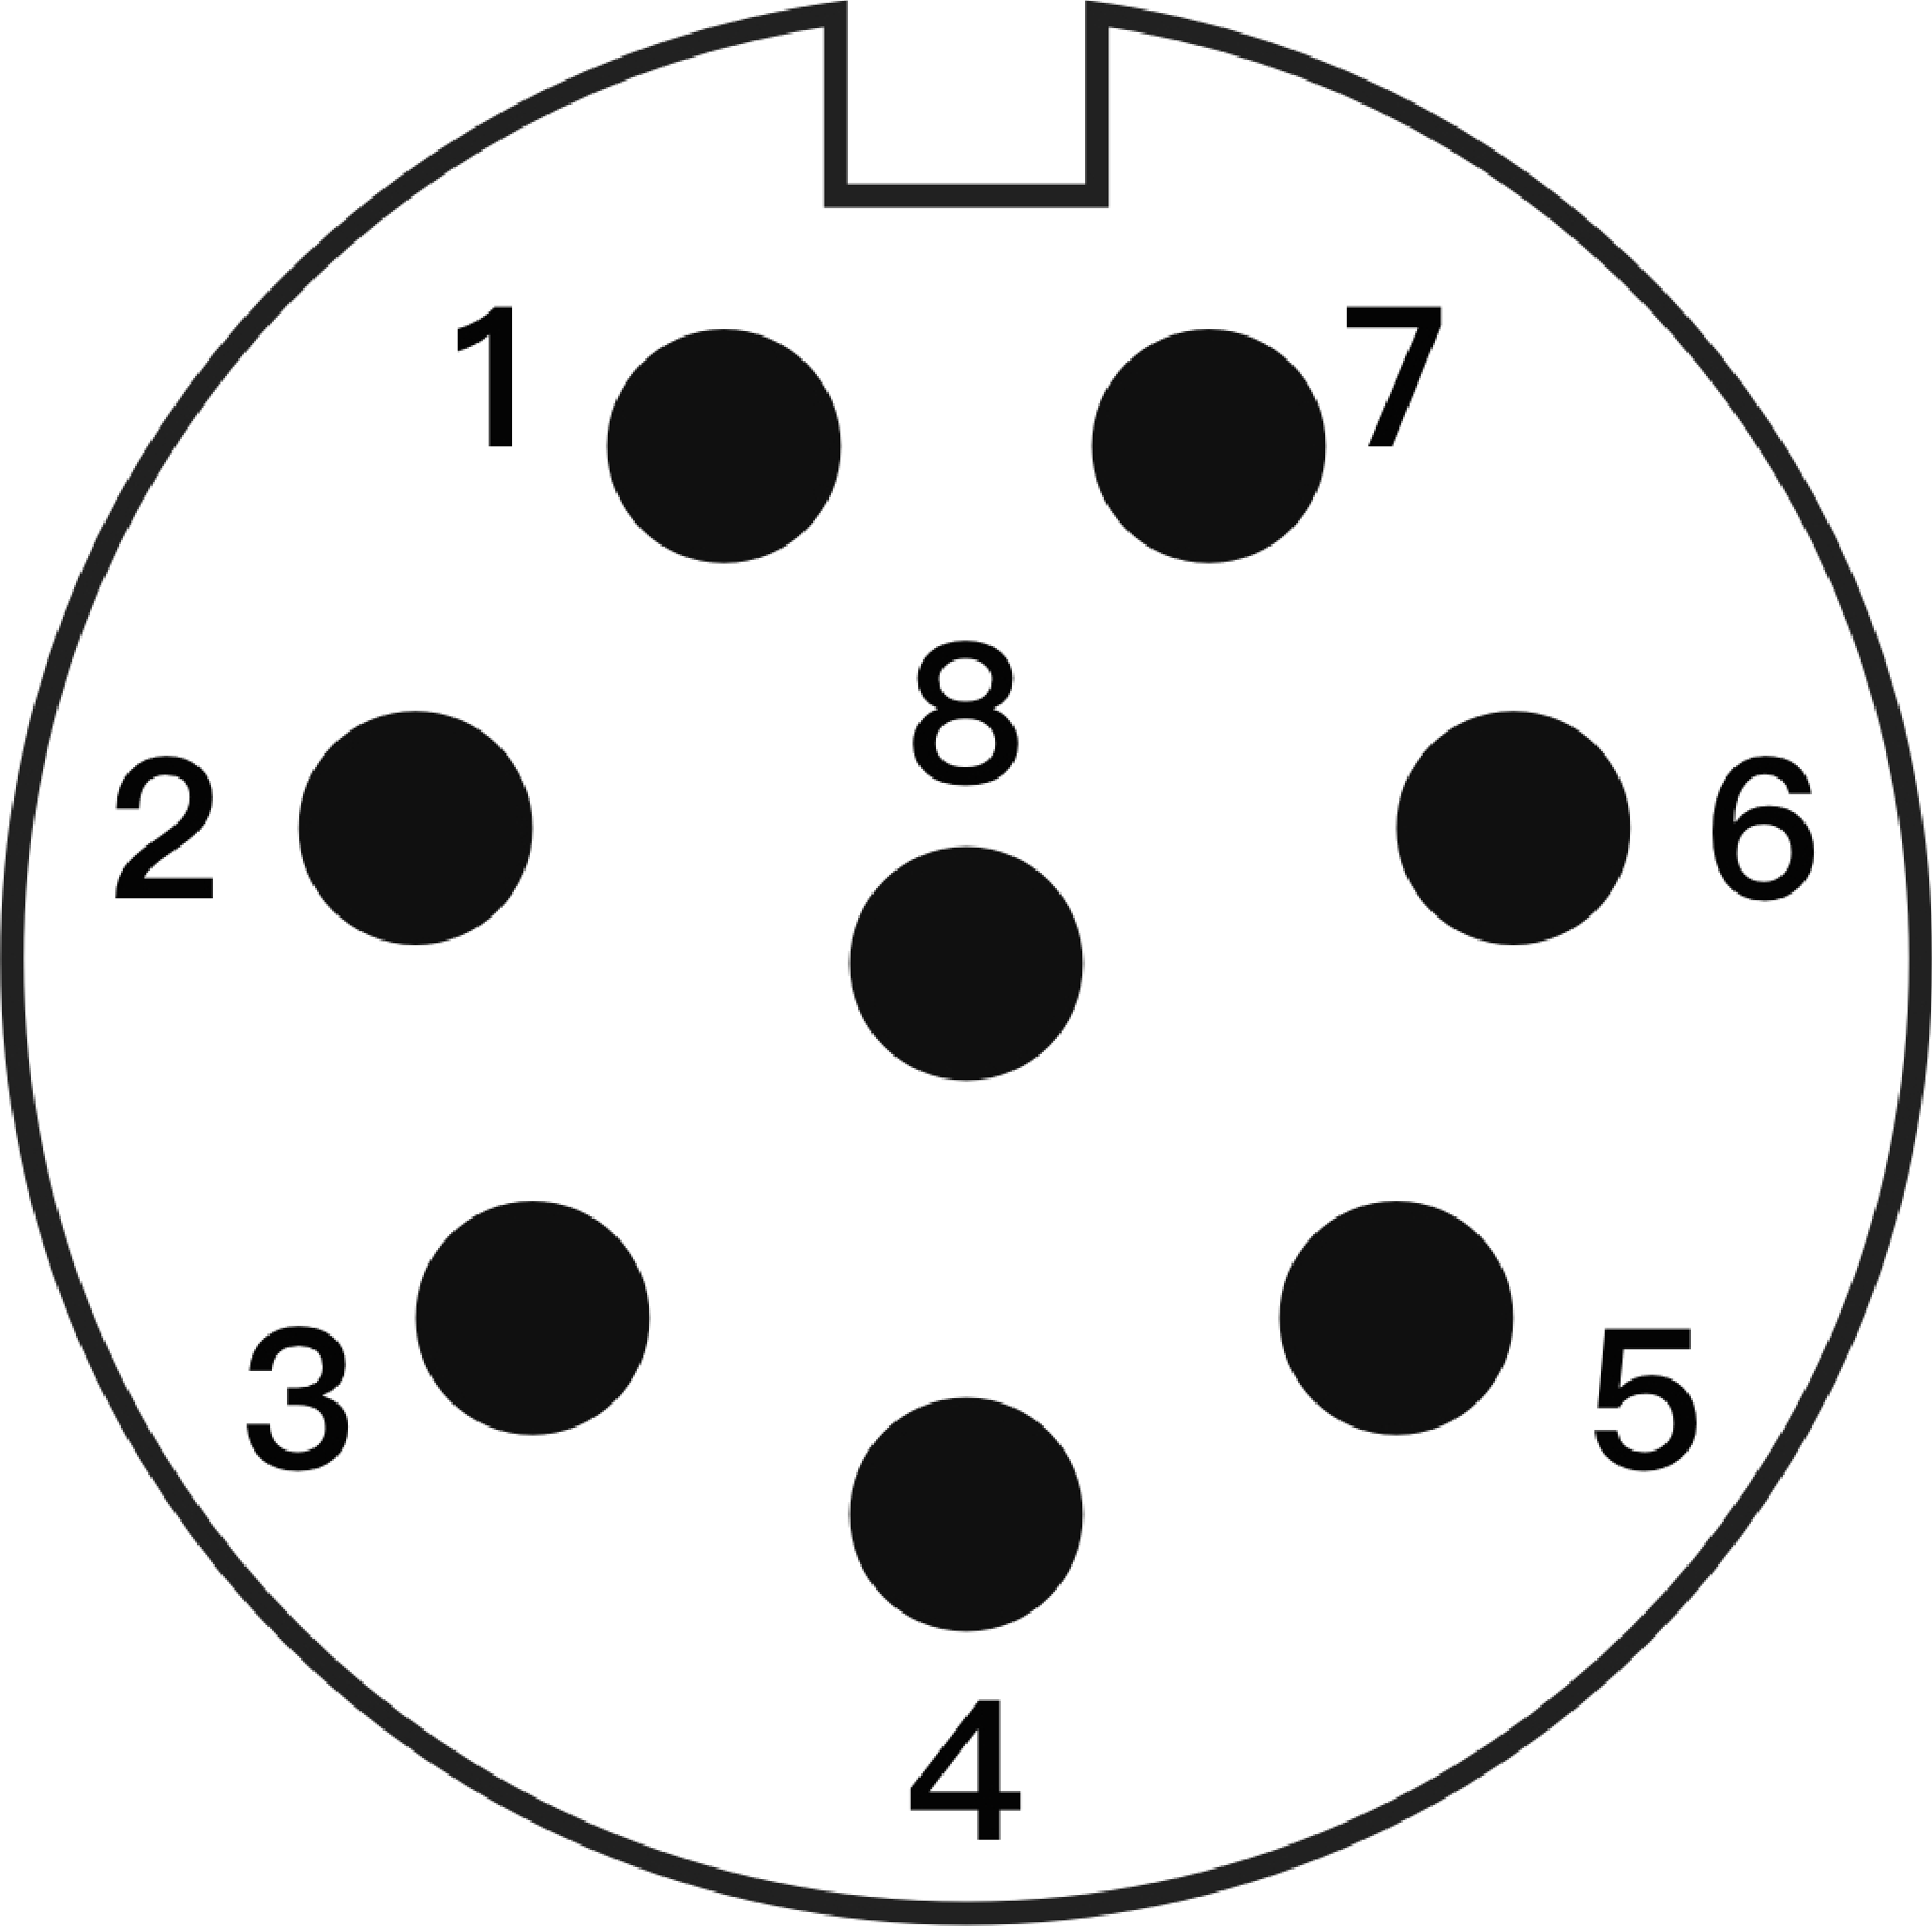
\includegraphics[height=3cm]{image/35.pdf}
    \caption{Schematic diagram of the flange I/O hardware port}
    \label{fig:法兰盘IO}
\end{figure}

\begin{table}[htb!]
    \centering
    \rowcolors{1}{trEven}{trOdd}
    \def\tE{\cellcolor{trEven}}
    \def\tO{\cellcolor{trOdd}}
\caption{Flange I/O description}
\begin{tabular}{cll}
   \rowcolor{th} \Th{Index}	&  \Th{Function}	& \Th{Parameters}\\
    1	&   Positive pole & \tO \\
    2	&   Negative pole & \multirow{-2}{5cm}{\tO
            Voltage $24\unit{V}$, Maximum current $2\unit{A}$    }\\
    3	&   Digital output 1	&  \tE \\
    4	&   Digital output 2	&   \multirow{-2}{5cm}{\tE PNP, output voltage $24\unit{V}$\\Total maximum current $1.5\unit{A}$}\\
    5	&   CANH	&  CAN bus high level \\
    6	&   CANL	& CAN bus low level  \\
    7	&   Digital input 1	&  \tO \\
    8	&   Digital input 2	&  \multirow{-2}{5cm}{\tO
            PNP, input voltage $3\sim 30\unit{V}$
    } \\
\end{tabular}
\label{tab:法兰盘IO}
\end{table}

\end{enumerate}

\clearpage

\section{Network Connection}

LM3 provides three different connection methods: Ethernet, Wi­Fi (2.4 GHz) hotspot network, and 4G IoT (Internet of Things) network. Ethernet and Wi­Fi network connections are provided for operating and connecting to robots. 4G IoT connections are currently only used for data reporting of device basic information\footnote{Equipment basic information is limited to: equipment name, equipment network connection type and status, software system version, system operation error information. Customer business data (including but not limited to scene data) is not included. The company will obtain your prior authorization and consent before reporting any other information.} (for device health monitoring).

% \vfill

% \clearpage

\section{Robot Installation}

As shown in \prettyref{fig:机器人安装方式}, the LM3 robot supports three install directions: up, down, and side (note that the robot cable outlet must face downwards when side­mounted).

\begin{figure}[htb!]
    \centering
    \subfigure[Up]{
		\begin{minipage}[b]{0.3\textwidth}\centering
			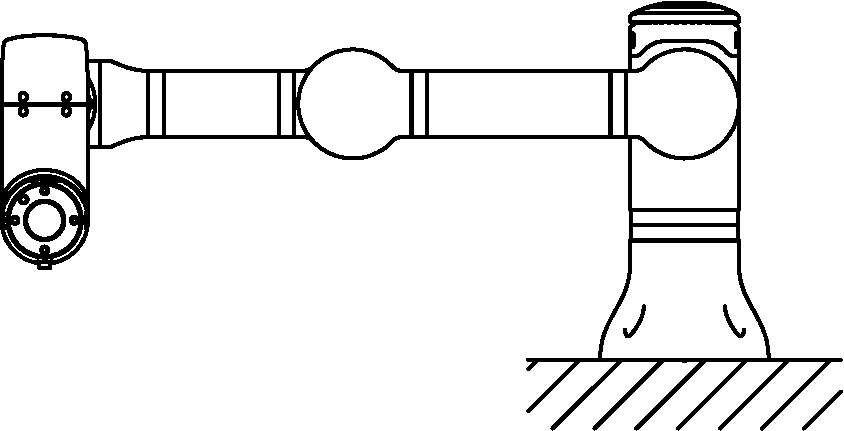
\includegraphics[width=\linewidth]{en/image/install_direction_up.pdf}
		\end{minipage}
	}
    \subfigure[Down]{
    	\begin{minipage}[b]{0.3\textwidth}\centering
   		 	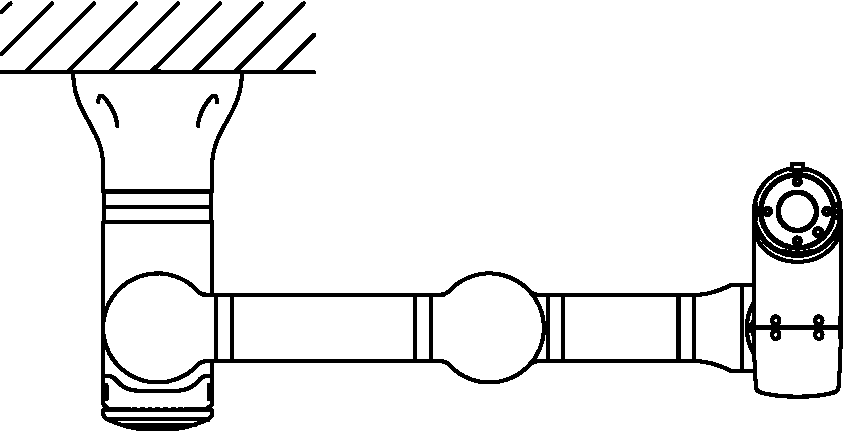
\includegraphics[width=\linewidth]{en/image/install_direction_down.pdf}
    	\end{minipage}
    }
    \subfigure[Side]{
    	\begin{minipage}[b]{0.3\textwidth}\centering
   		 	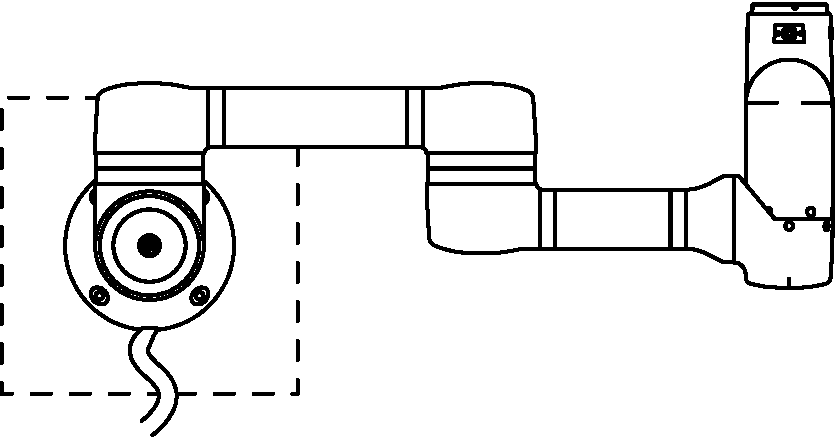
\includegraphics[width=\linewidth]{en/image/install_direction_side.pdf}
    	\end{minipage}
    }
    \caption{Installation mode of the robot}
    \label{fig:机器人安装方式}
\end{figure}

% \clearpage

% \vspace*{-0.6cm}

Use the 4 M6 screws in the robot accessory kit to correspond to the 4 mounting holes on the robot base (\prettyref{fig:机器人底座视图}). It is recommended to tighten these screws with a torque of $9\Nm$. If you need to adjust the robot position more accurately, you can also drill 2 holes with a diameter of $5 \mm$ and fix them with pins.

% \vspace*{-0.8cm}

\begin{figure}[htb!]
    \centering
    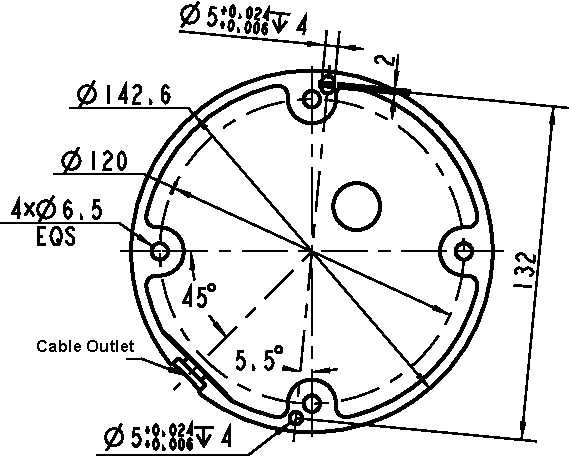
\includegraphics[height=5cm]{en/image/bottom_surface.pdf}
    \caption{Robot base view}
    \label{fig:机器人底座视图}
\end{figure}

\info{\begin{itemize}
\item Fix screws in all mounting holes of the robot.
\item During the installation, hold the robot until all the screws on the base are tightened.
\end{itemize}}

\danger[WARNING]{Do not fix the robot (including the control box) in an unstable position, otherwise it may fall and thus damaged.}

\clearpage

\section{End-Effector Installation}

As shown in \prettyref{fig:机器人末端法兰盘接口}, there are 4 M6 threaded holes on the front of the end flange of the robot, which are used to connect the end-effector and the robot;
there are 4 M3 threaded holes on the side of the flange, which are used for the installation of Lebai lightweight end-effector. Under normal use and excluding external collisions, the end of the robot (including effectors) can bear a maximum load of $3\kg$.

\begin{figure}[h!]
    \centering
    \subfigure{
		\begin{minipage}[b]{0.2\textwidth}\centering
			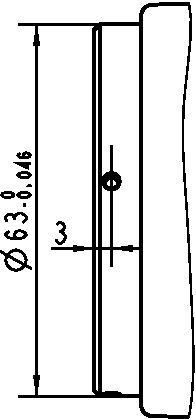
\includegraphics[height=4cm]{en/image/flange_side_view.pdf}
		\end{minipage}
	}
    \subfigure{
    	\begin{minipage}[b]{0.5\textwidth}\centering
   		 	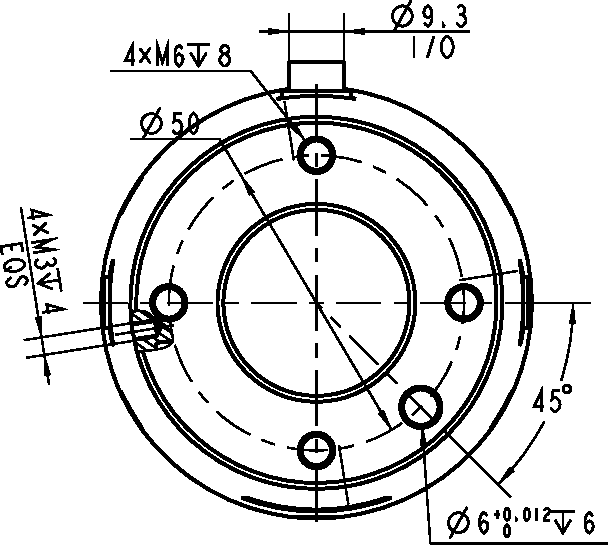
\includegraphics[height=4cm]{en/image/flange_face_view.pdf}
    	\end{minipage}
    }
    \subfigure{
    	\begin{minipage}[b]{0.2\textwidth}\centering
   		 	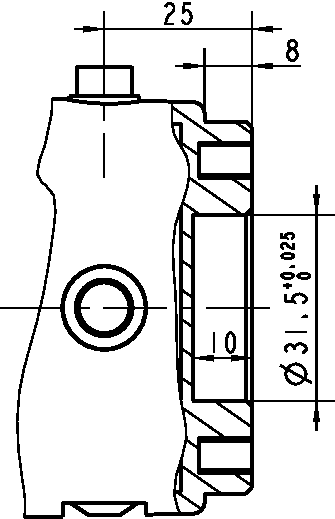
\includegraphics[height=4cm]{en/image/flange_top_view.pdf}
    	\end{minipage}
    }
    \caption{Robot end flange port}
    \label{fig:机器人末端法兰盘接口}
\end{figure}

% \clearpage

\NoBgThispage

\begin{figure}[htb!]
	\centering
	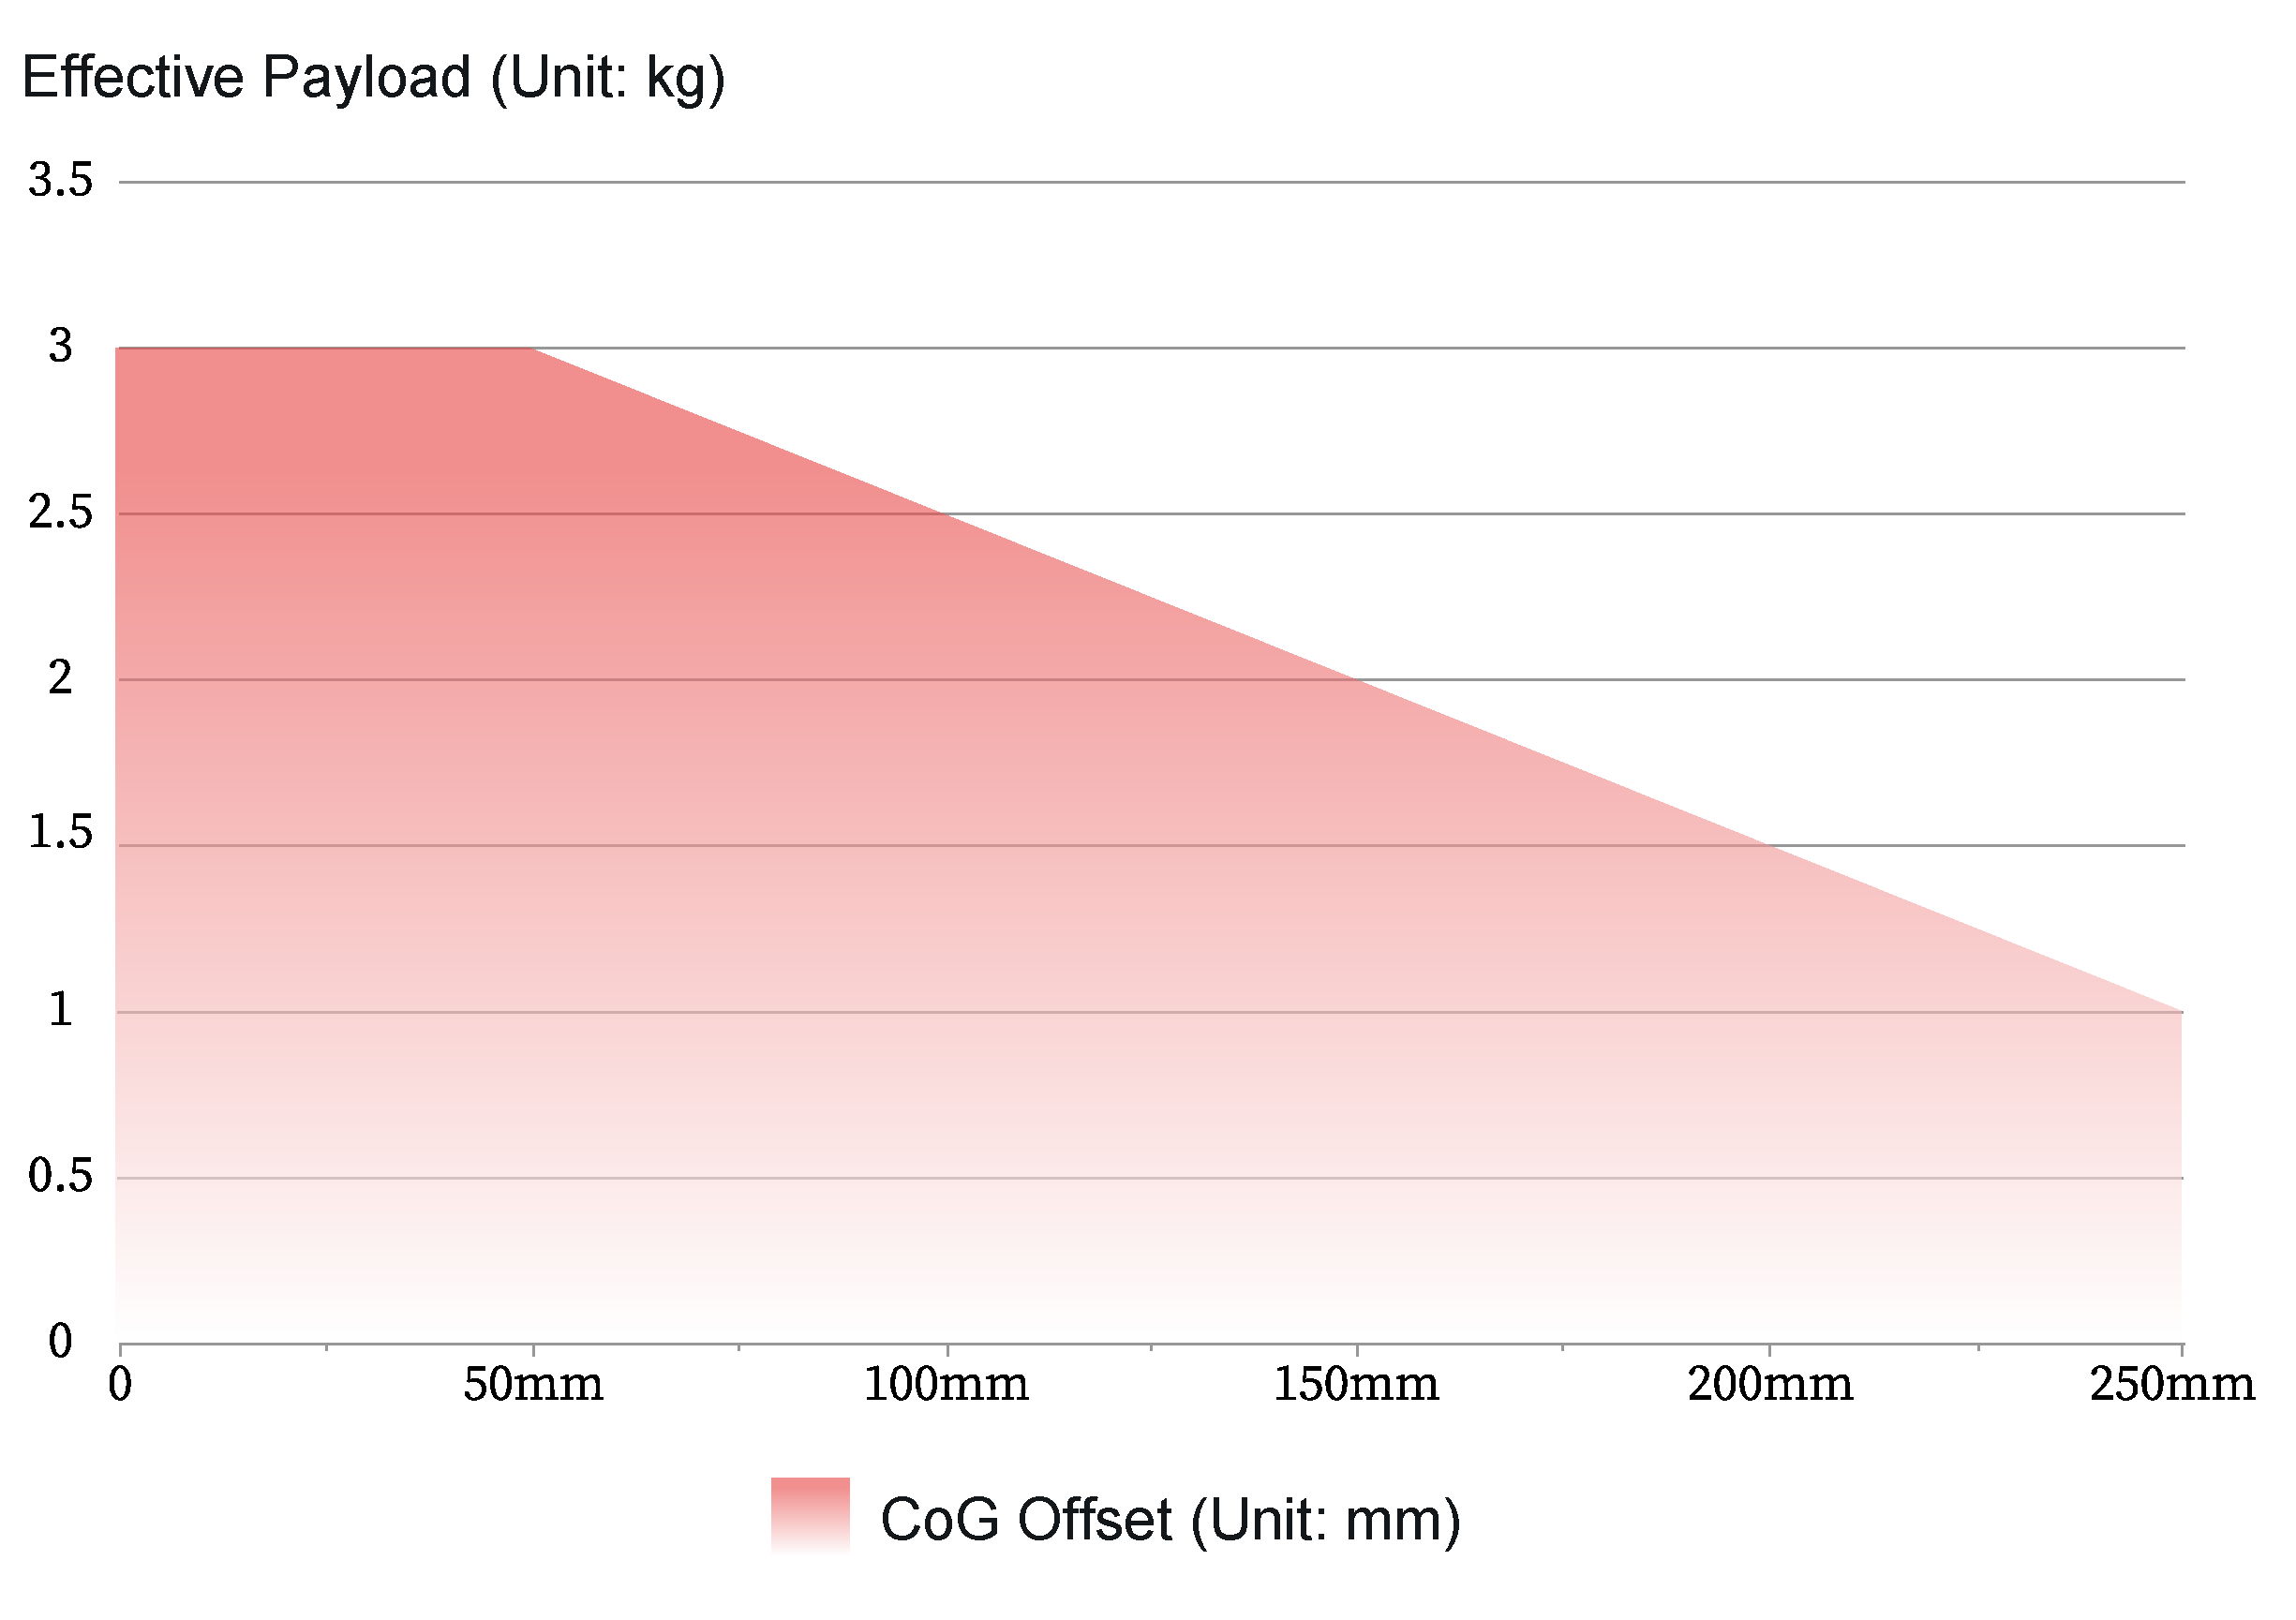
\includegraphics[width=\textwidth]{en/image/effective_payload.pdf}
	\caption{Effective payload}
	\label{fig:有效负载图}
\end{figure}

The maximum allowable payload of the robot depends on the center of gravity (CoG) offset, see \prettyref{fig:有效负载图}.
% 重心偏移定义为工具输出法兰的中心与重心之间的距离。
The CoG offset is defined as the distance between the center of the effector output flange and the CoG.

\danger[WARNING] {\begin{itemize}
	\item The load condition should be within the range shown in the chart.
	\item The effective load shown in the chart indicates the maximum load capacity. Under no circumstances should it exceed the maximum weight shown in the chart.
	\item Exceeding the max effective payload will cause premature damage to the internal parts of the robot.
\end{itemize}}